\label{chap:p4-imrt_study}
\section*{Preamble}
Following the full characterization of the measurement system (Chapter~\ref{chap:p1-system}) and the spectrally-constrained model (Chapter~\ref{chap:p3-model}), a study was devised to employ both in the clinical setting. In radiation therapy, it is common to compare two treatment or skin care management regimens using only visual assessment (VA) and patient questionnaires. Both of these evaluation techniques are subjective in nature, meaning that there is a large amount of inter- and intra- observational variation. The spectrally-constrained integrating sphere-based diffuse reflectance spectroscopy approach outline in the previous papers provides a quantitative, objective way to quantify patient skin reactions. However, it is not as easily implemented as VA.

This paper explains where the difficulty in implementation comes from, and how it can be best addressed. This is a very important step in making the system and accompanying model accessible to the clinical community. More clinicians may adopt this assessment method if they have a set of recommendations on how it should be used to optimize clarity in the results.

This study required research ethics board (REB) approval. The application was prepared by the author of this thesis (further known as ``the author'') with significant assistance from Mrs. L. Doerwald-Munoz and under the guidance of Drs. T. Farrell, J. Hayward, O. Ostapiak, and J. Wright. The daily measurements were very time-consuming and required much assistance from Mrs. Doerwald-Munoz with occasional help from Miss. C. Cook and Dr. P. Muruganandam. All analysis was performed by the author. The manuscript was written by the author under the guidance of Drs. Farrell and Hayward and was additionally editted by the other authors, Drs. Ostapiak and Wright, and Mrs. Doerwald-Munoz. The manuscript has been altered from its original form to match the style of this thesis.

\section*{Contents}

\begin{center}
	
	\textbf{Diffuse reflectance spectroscopy for monitoring erythema in head \& neck intensity modulated radiation therapy}
	
	Diana L. Glennie, Joseph E. Hayward, Orest Z. Ostapiak, James Wright, Lilian Doerwald-Munoz, and Thomas J. Farrell
	
	\textit{Department of Medical Physics and Applied Radiation Sciences, McMaster University, 1280 Main Street West, Hamilton, Ontario, L8S 1A8}
	
	\textit{AND}
	
	\textit{Department of Medical Physics, Juravinski Cancer Centre, 699 Concession Street, Hamilton, Ontario, L8V 5C2}
	
\end{center}

\noindent Submitted to the \textit{Journal of Radiation Oncology} on November 5, 2014.

\section*{Abstract}
\noindent \emph{Objectives} To outline the best practices for obtaining and interpreting quantitative measurements of erythema in radiation therapy patients with a diffuse reflectance spectroscopy (DRS) system.

\noindent \emph{Methods} Ten patients receiving intensity modulated radiation therapy (IMRT) for head \& neck cancer were enrolled in a prospective observational study. Prior to the delivery of each fraction of radiation, DRS measurements were recorded. In addition, weekly dose measurements and visual assessments were performed. The daily variation in the total hemoglobin in skin was determined and used to identify the first day of significant increase in total hemoglobin. The impact of measurement frequency and data smoothing was investigated.

\noindent \emph{Results} The daily variation in the total hemoglobin in a control region of skin was found to be 15.6\% (st. dev.). To reduce the impact of this on serial erythema measurements, a 3-point centered moving average was applied. The range of maximum increase in the relative total hemoglobin concentration for the patients in this study was 36-254\%. The daily variation in the total hemoglobin was used to calculate a minimum detectable increase threshold. It was possible to detect skin redness from 1 to 19 days before visual assessment.

\noindent \emph{Conclusion} DRS offers a quantitative alternative to the subjective visual assessment method of evaluating radiation-induced erythema. It can be easily implemented into interventional studies to compare patient skin response.

\section{Introduction}
Intensity Modulated Radiation Therapy (IMRT) is the standard of care for head and neck (H\&N) cancers as it is capable of delivering the prescribed dose to the tumor target while sparing nearby radiosensitive organs.\cite{Lee2007} However, H\&N IMRT is often accompanied by higher rates of acute toxicity in the treatment field, commonly in the form of erythema, that can often be severe and painful for the patient.\cite{DeConno1991} The prevailing hypothesis is that the thermoplastic masks, required for patient immobilization, have a bolus-like effect on the skin.\cite{Lee2002} In addition, since skin is hard to contour in the treatment planning software, the true skin dose is usually underestimated.\cite{Court2008} Moreover, since skin is not considered to be a radio-sensitive organ, its dose is not always purposefully minimized.\cite{Saibishkumar2008}

Radiation-induced erythema, or radiation dermatitis, begins as an inflammatory response to the destruction of  basal cells in the epidermal layer of skin that results in the cells migrating to the surface at an increased rate.\cite{McQuestion2006} Since erythema is a deterministic effect there is a threshold dose and, following incidence, the severity increases with dose. Acute erythema typically appears two to three weeks following the start of IMRT and peaks around five weeks into treatment. In addition to the patient-specific response, erythema also depends on the volume of tissue involved. Due to these many factors, it is impossible to reliably predict the extent and latency period of a specific patient’s reaction.\cite{Porock2002}

Erythema can be extremely painful and there is a risk of infection. Severe cases of erythema may lead to an interruption in the treatment delivery, possibly compromising the treatment efficacy.\cite{Maciejewski1989} There is also a risk of permanent damage such as skin discoloration due to the migration of the melanocytes to the more superficial layers of the epidermis,\cite{McQuestion2006} or tissue necrosis which may occur up to 2-4 years following the radiation treatment.\cite{Lee2002} Therefore, it is important to properly monitor and manage a patient’s skin response.

Radiation-induced erythema is commonly managed with proper hygiene and skin care.\cite{McQuestion2006} Patients are often prescribed a topical treatment to soothe the skin and potentially minimize the reaction. In reviews on skin-care management for radiation therapy patients, nearly all of the reviewed studies relied on visual assessment (VA) (along with patient questionnaires) to compare the efficacies of the two management regimens.\cite{McQuestion2006,Wong2013,Chan2014} With VA, the skin area of interest is observed by a researcher and classified using one of any number of skin reaction scales. These scales can be divided up into two main types; those with four or fewer classifications,\cite{Wan1983a,Cox1995,Lock-Andersen1998,Kirova2011} and those with more.\cite{Pearse1990,Wengstrom2004,Bodekaer2013} Scales with four or fewer classifications are not precise enough to differentiate between the various levels of erythema. For example, the prevalent Common Terminology for Adverse Events (CTCAE v4.03)[19] has four categories ranging from faint/dull erythema to complete necrosis. Patients experiencing skin reactions will continue to be classified as a “1” until moist desquamation is observed. Although this scale is easier and more consistent to use, it does not provide enough information for comparison purposes. Scales with greater than four classifications are able to capture the different stages of an erythematic response (e.g. “mild” vs “moderate” levels), but there will be large inter- and intra- observer differences when comparing between different days, observers, and studies. These scales are also more difficult to use for more heavily pigmented individuals in which an increase in skin redness may not be easily observed.

In an effort to establish a quantitative evaluation technique, recent work has focused on using diffuse reflectance spectroscopy (DRS) to monitor skin redness. DRS relies on the properties of both oxy- and deoxy-hemoglobin that allow them to preferentially absorb green light. When skin appears redder to the human eye, it is not because more red light is being reflected, but because less green light is being scattered back out of the tissue (see Figure~\ref{fig:p4-drs_example}). Therefore, as the concentration of hemoglobin increases, more green light is absorbed. Previous systems commonly used only two small ranges of wavelengths (one red, and one green) to measure skin redness,\cite{Pearse1990,Dawson1980,Diffey1984,Feather1988} but they were unable to account for the effect of melanin on the reflected light intensities. More recent systems use the entire visible light spectrum.\cite{Stamatas2008,Yohan2014,Kollias2010} Hemoglobin is located in the dermis, below the melanin-containing epidermis. Since the thickness and melanin-content of the epidermal layer is unknown, the recovered hemoglobin concentrations from any reflectance method are apparent concentrations for a homogeneous single layered tissue and not the true concentrations found in the dermal layer. These results can, however, be accurately expressed as a percent difference from a baseline measurement.

\begin{figure}
	\centering 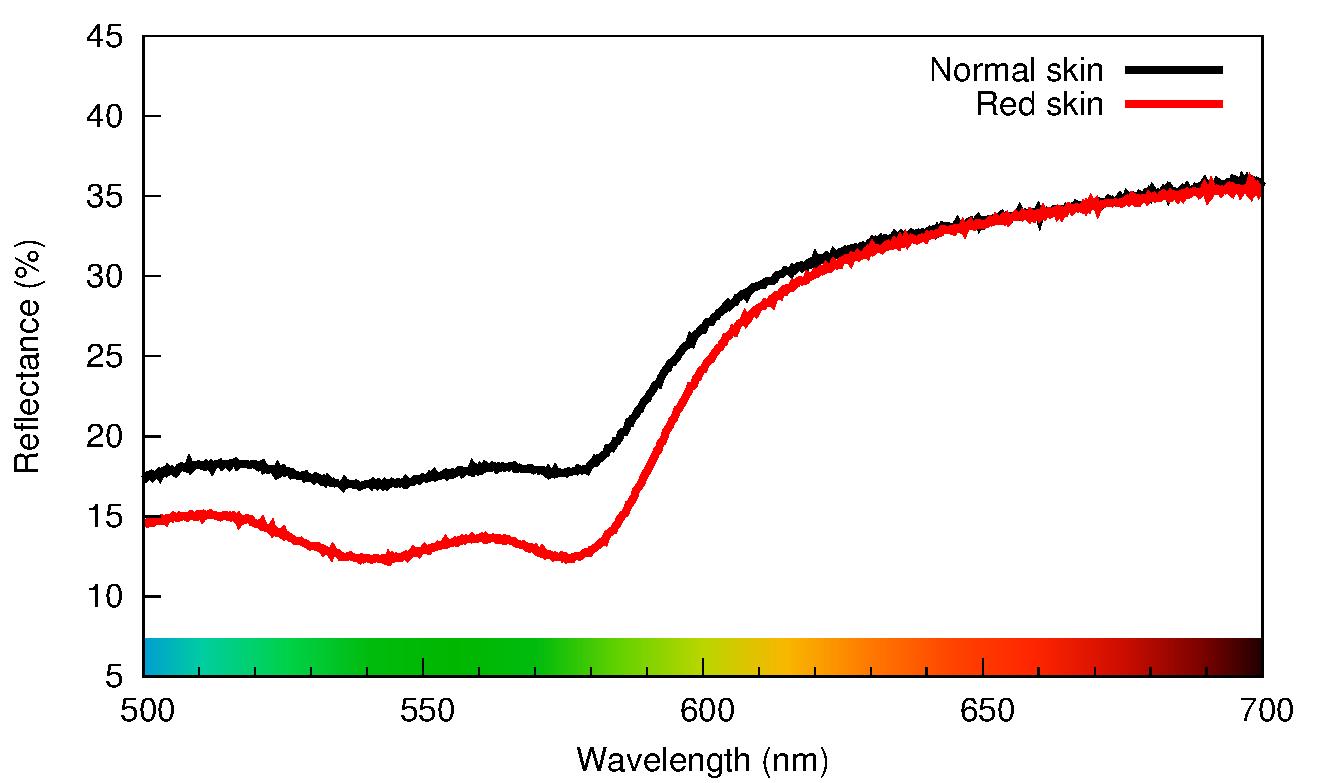
\includegraphics[width=0.6\textwidth]{figures/p4-drs_example.png}
	\caption[Example of the diffuse reflectance spectra for normal and red skin]{\label{fig:p4-drs_example}Total diffuse reflectance spectra for the same area of skin before and after the inducement of skin reddening. The amount (percent) of red light is the same for both measurements but there is a decrease in the amount of green light reflected from the reddened skin.}
\end{figure}

While qualitative evaluations, such as VA, have a straight-forward implementation due to their simplicity, quantitative approaches, such as DRS, require more thorough consideration prior to use. This is primarily due to the daily variation in the blood concentration of skin. Although there is no consensus on the diurnal variation, a review by Brown et al. found it to be on the order of 10\% with a maximum ranging from 15 to 30\%.\cite{Brown1946} While these changes in concentration levels may not be visibly detected, they will likely appear in the quantitative measurements, making it difficult to interpret trends in the recovered hemoglobin concentrations.

The purpose of this article is to outline the best methods for collecting data with a DRS system, as well as describe how to process the results to improve interpretation. This objective was achieved through a prospective, observational study in which patients treated with IMRT underwent daily DRS measurements over the course of their treatment. From the collected data, the daily variation in the reflectance of non-irradiated skin was established. This result was then used to establish the optimum measurement frequency and what (if any) data smoothing should be applied. Finally, the first day of measurable skin redness was identified for each volunteer following the newly established approach and was compared to the date of the first erythema note from the patient charts.

\section{Materials \& Methods}

\subsection{Subject Selection}
Patients at the Juravinski Cancer Centre (Hamilton, Ontario, Canada) were eligible for inclusion in the study if they were receiving IMRT for a head and neck cancer between October 2010 and March 2011. Prescribed radiation doses were either 60 or 70 Gy, given daily at a rate of 2 Gy per fraction. None of the enrolled participants were receiving concurrent chemotherapy. A total of 14 volunteers were enrolled, with 10 successfully completing the study. Four of the participants did not complete the study due to personal reasons or health concerns. Of those that successfully completed the study, one volunteer was retroactively removed due to bolus modification during the course of treatment. In total, nine complete data sets were collected. Completed volunteers were all Caucasian males between the ages of 41 and 79, although neither gender, nor age, nor race were screening criteria. Hamilton Health Sciences Research Ethics Board approval was obtained for this prospective study.

\subsection{Measurement System}
The diffuse reflectance spectroscopy system used in this study has been discussed elsewhere.\cite{Glennie2014a} Briefly, the measurement area is illuminated with white light delivered through a highly reflective integrating sphere. Light reflected back into the sphere is collected by an optical fiber and delivered to a spectrometer. The collected spectrum is then processed to extract a total hemoglobin concentration\cite{Glennie2014b} which is expressed as a percent difference from an established baseline measurement.

\subsection{Study Protocol}
Prior to the first fraction of radiation and the first DRS measurement, participants’ radiation treatment plans were assessed to determine the location of the projected maximum skin dose. A measurement location was chosen on the skin that was close to this area while being sufficiently flat to ensure good contact between the collection port of the measurement device and the skin. The location was marked on the skin with an indelible marker to ensure daily placement accuracy. A back-up template was also created on an 8.5 inch x 11 inch transparency film, using topographical landmarks such as freckles, moles, and scars for alignment. A patch of skin was selected outside of the radiation field on the upper lateral portion of the left arm that was relatively free of hair and other irregularities to collect control data.

Before each fraction of radiation, participants were escorted to a private room and asked to sit quietly for 5 minutes in an attempt to reduce the effects of vasodilation due to exertion and external temperature exposure. Three measurements were then taken on the arm, followed by three measurements on the head/neck. The entire collection procedure lasted less than 15 minutes. No fractions were delivered on weekends or statutory holidays.

Weekly questionnaires were used to monitor changes in participant behavior that might affect the study results, such as voluntary sun exposure and any skin care regimens. VAs of the volunteer skin conditions were performed by the attending oncologists during their weekly patient assessment. Each week, thermoluminescent detectors (TLDs) arrays were placed inside patient masks over the DRS measurement areas to determine the skin dose received per fraction.

\subsection{Data Analysis}
For each day and measurement location (head/neck and arm), the three measured spectra were averaged to increase the signal to noise ratio.\cite{Fullerton1996} Each averaged spectrum was background subtracted and normalized to a calibration measurement in order to obtain reflectance spectra. These were then analyzed to recover the total hemoglobin concentration. The first measurement (taken prior to the first fraction of radiation) was assigned as the baseline and all subsequent measurements were expressed as a percent difference from this value.

\section{Results \& Discussion}

\subsection{Variation in DRS Measurement \& Minimum Detectable Difference in Blood Concentration of Hemoglobin}
Previously, the DRS system was characterized and was able to recover chromophore concentrations to within 5\% in tissue-simulating phantoms.\cite{Glennie2014b} However, the daily variation of the hemoglobin concentration in skin has been reported as low as 2\% and as high as 30\%.\cite{Brown1946} Therefore, the measurements performed on volunteer arms were analyzed to determine the daily variation for this particular study sample.

The measurement location on the arm was well outside of the treatment field and as such, was not expected to vary appreciably over the course of treatment. However, there may have been slight variations in the hemoglobin concentrations over time from external factors such as environmental temperatures. To account for this possibility, the measured hemoglobin for each individual patient (expressed as a percent difference from the first measurement) was plotted against time and a straight line was fit to these data and subtracted to obtain the residuals (See Figure~\ref{fig:p4-daily_var} for data from a representative patient).

\begin{figure}
	\centering 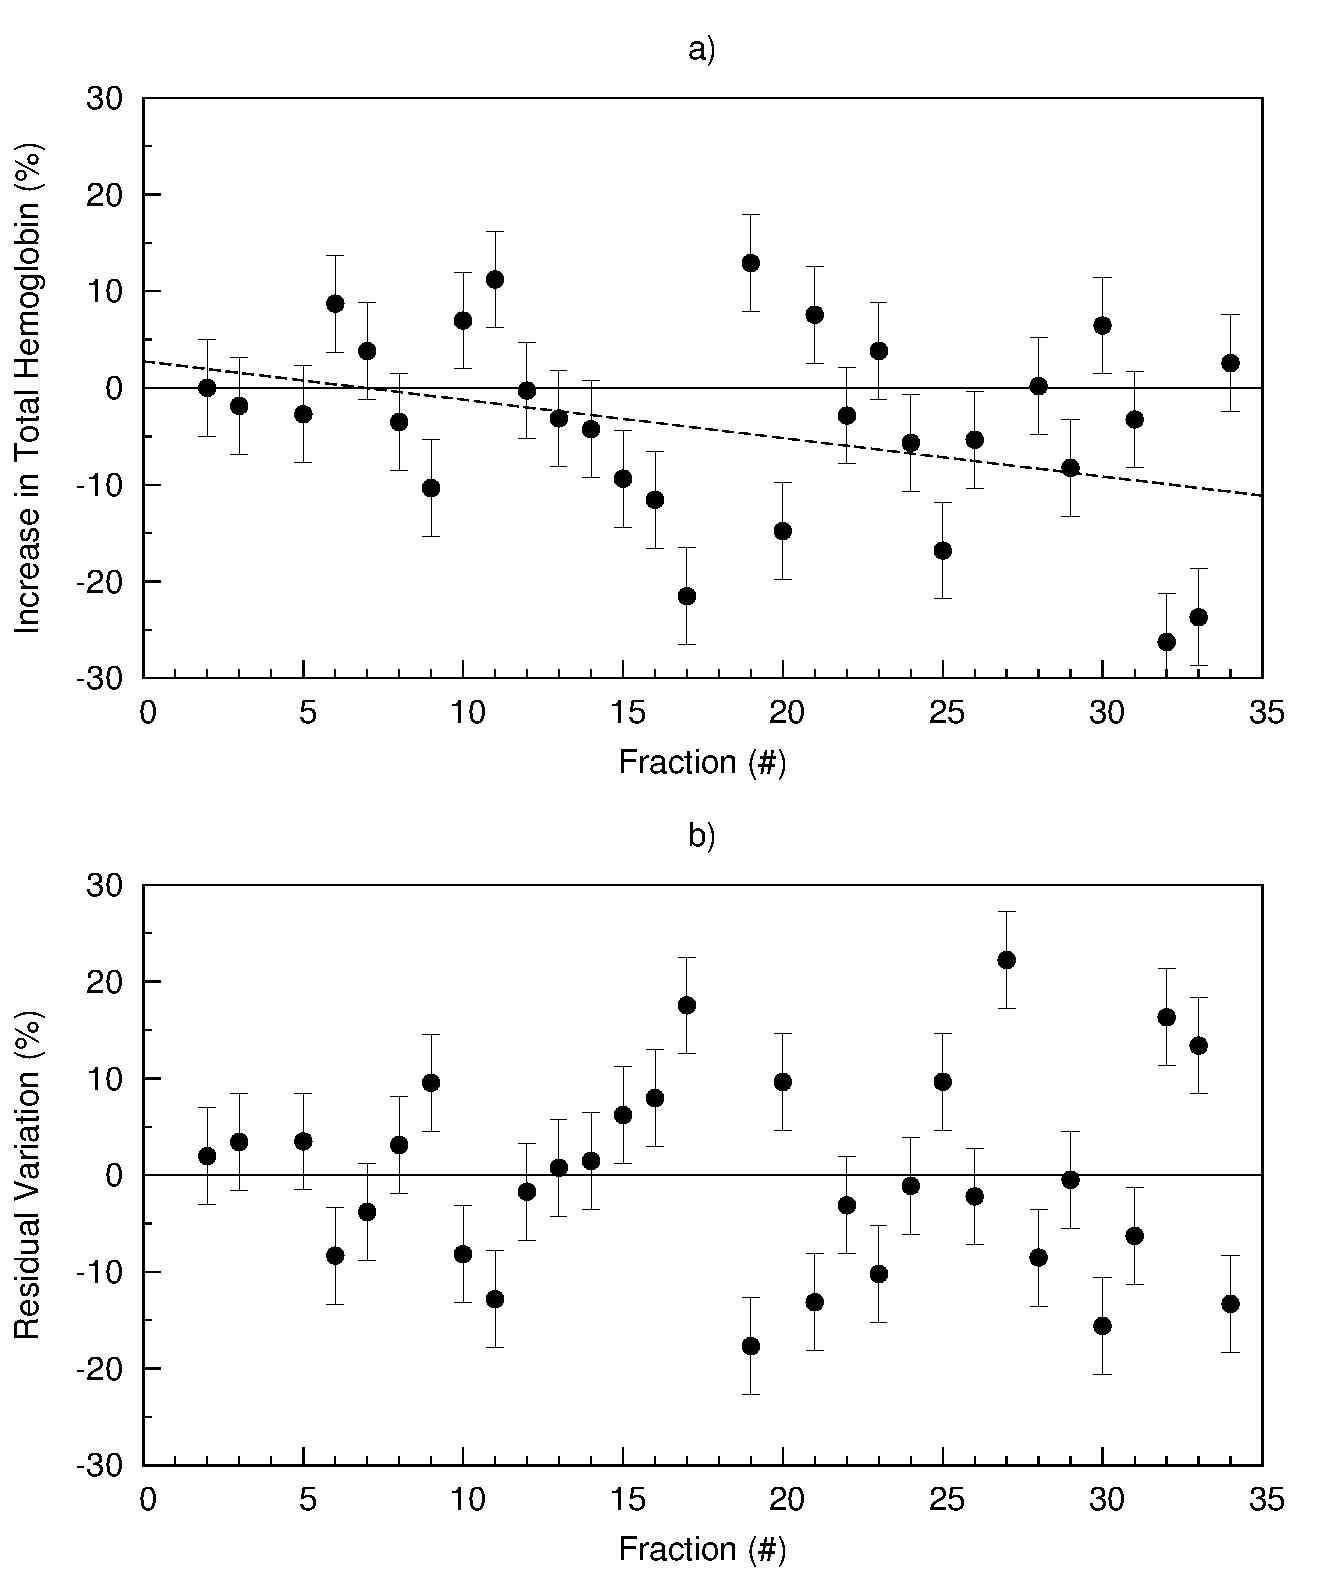
\includegraphics[width=0.6\textwidth]{figures/p4-daily_var.png}
	\caption[Sample daily variation of hemoglobin in control site]{\label{fig:p4-daily_var}a) The total hemoglobin at the control site, expressed as a percent difference from the first measurement for a typical patient along with a linear fit. b) The residuals when the measurements were subtracted from the line of best fit.}
\end{figure}

The standard deviation in the percent difference in hemoglobin concentration for each volunteer was calculated. The typical, or population, standard deviation for the patients in the study was 15.6\%.\cite{Knight1999} A minimum detectable difference in hemoglobin concentration could be defined as the 95\% confidence interval for this population.  Since only an increase in total hemoglobin concentration in the form of erythema is under investigation, the 95\% confidence interval for a one-tailed test can be determined from the 90\% confidence interval (1.64*st. dev.) for a two-tailed test. Thus, the minimal detectable increase (MDI) is 25.6\%.

\subsection{Skin Erythema Measurements}
Skin erythema measurements were collected daily at the treatment site and were processed as a percentage difference from the first result. Figure~\ref{fig:p4-combined_fig}a shows the daily measurements from one study volunteer with the MDI, plotted as a dotted line. While the daily variation makes it difficult to interpret, there is a noticeable increase in the total hemoglobin over time. However, there are also many excursions of the data across the MDI threshold.

\begin{figure}
	\centering 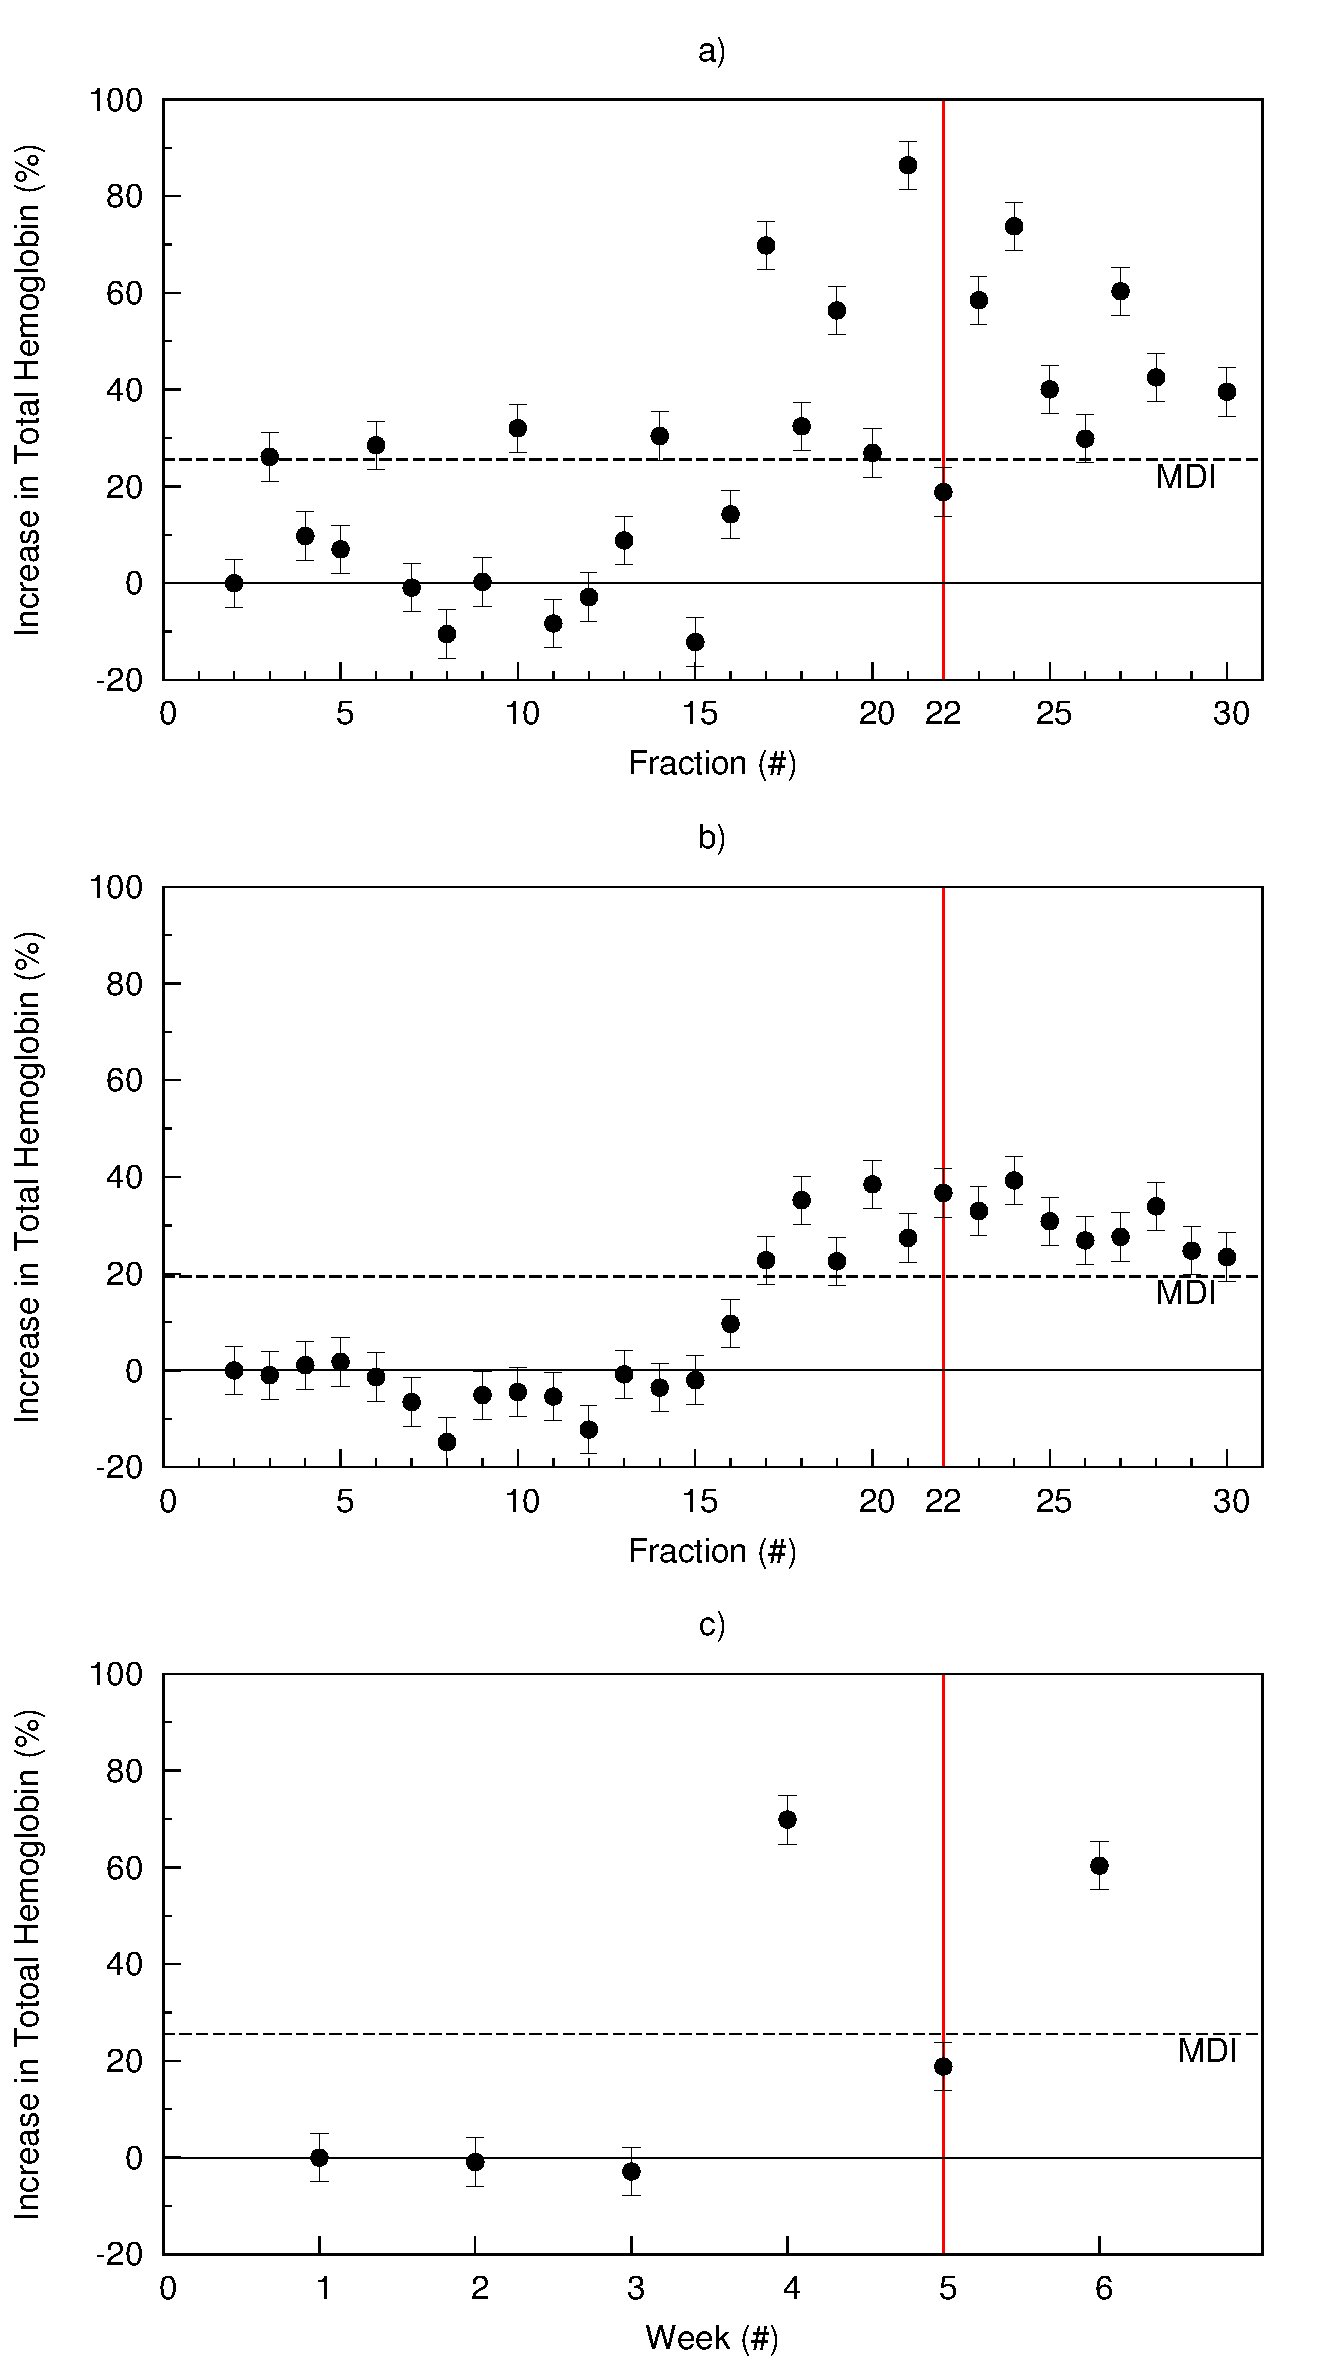
\includegraphics[width=0.6\textwidth]{figures/p4-combined_fig.png}
	\caption[Increases in total hemoglobin concentration for a representative patient]{\label{fig:p4-combined_fig}a) Daily total hemoglobin measurements expressed as a percent difference from the first measurement for a typical volunteer. b) The same data with a 3-point centered moving average applied and a recalculated MDI threshold. c) One of every five data points from the same volunteer representing weekly measurements. For this volunteer, erythema was first noted visually on Fraction 22/Week 5 as indicated by the red line.}
\end{figure}

To improve the interpretation of the results, some form of data smoothing was considered. Since the percent increase in total hemoglobin is a scalar observation recorded over time with a constant measurement interval, data smoothing techniques for univariate time series were considered to improve the diagnostic value of the data.\cite{Prins2013} A moving average is the most common smoothing filter for time series analysis. It reduces the daily variation in the total hemoglobin concentration and can highlight any long term trends in the data. The period of the moving average should be relatively short, based on the total number of observations made. If using a centered instead of a leading moving average, odd numbered periods work best. On the scale of 30-35 measurements, a moving average of three should provide sufficient smoothing without obscuring possible smaller trends (e.g. weekly trends). Given the amount of daily variation in the measurements and the chosen period, there is no significant improvement in the data smoothing when employing a weighted moving average over a simple moving average (data not shown). Therefore, a 3-point centered moving average (3PCMA) was applied to the data collected in this study.

Since a moving average decreases the magnitude of the daily variation, the MDI was recalculated. The control measurements were reprocessed with a 3PCMA and the percent standard deviation was determined to be 11.8\%. This value was confirmed by applying quadrature error propagation to the previously determined percent standard deviation. Using the same confidence interval as before, the MDI for the 3PCMA smoothed data was found to be 19.4\%. The data from Figure~\ref{fig:p4-combined_fig}a is shown with a 3PCMA smoothing filter and the new MCI in Figure~\ref{fig:p4-combined_fig}b.

For the patient data shown in Figure~\ref{fig:p4-combined_fig}b, the percent increase in total hemoglobin remains relatively constant at the baseline concentration from the first fraction’s measurement. It begins to increase around fraction 15, corresponding to the third week of treatment. This is consistent with the clinically observed trends discussed in the introduction. Following this change, the percent increase in total hemoglobin levels off above the MDI threshold at approximately 40\%. Similar trends were seen in all the study volunteers. For patients where the percent increase in total hemoglobin exceeded the MDI, the range of maximum erythema levels was 36-254\%. The majority of papers that monitored UV-induced erythema did not analyze the results in a similar way and cannot be used for comparison,\cite{Harrison2002,Wagner2002,Wong2010} except for Stamatas et al.\cite{Stamatas2008} who reported a range of (dose dependent) relative increase in oxy-hemoglobin of 4-237\%. In the lone study on radiation-induced erythema, Yohan et al.\cite{Yohan2014} exposed nude mice to a single fraction of 40 Gy and recovered relative increases in total hemoglobin concentration of 14-256\%.

If the MDI is used to indicate the point at which skin redness is distinguishable from daily fluctuations, the first signs of erythema should be visually identified on Day 17 for this specific volunteer – five days prior to the actual visual identification. Table~\ref{tab:va_vs_mdi} shows a summary of the number of fractions leading up to the identification of erythema with both the visual and MDI methods. For seven of the nine volunteers, the MDI assessment method identified erythema earlier than the visual method. In one volunteer, no notes were made in the patient chart regarding skin redness, although the MDI method did detect skin redness during treatment. In another volunteer, the MDI threshold was never reached in the DRS measurements although a note identifying erythema was made in the patient chart. For this particular volunteer, the visual identification was made during the fourth week of treatment. Given that the skin dose was relatively low (55 cGy/frac), the visually noted erythema may be due to empirical bias. While it should be reiterated that oncologists only saw patients once a week for VA, the MDI detection method preceeded the visual detection method by more than five fractions (i.e. one week) for the majority of volunteers.

\begin{table}[h]
			\centering
			\caption{Days until the first assessment of erythema using visual identification and the MDI threshold.}
			\label{tab:va_vs_mdi}
	\begin{tabular}{cccccccccc}
		\hline
		\multicolumn{1}{|c|}{Volunteer}                                                           & \multicolumn{1}{c|}{1}   & \multicolumn{1}{c|}{2}   & \multicolumn{1}{c|}{3}   & \multicolumn{1}{c|}{4}  & \multicolumn{1}{c|}{5}   & \multicolumn{1}{c|}{6}   & \multicolumn{1}{c|}{7}   & \multicolumn{1}{c|}{8}   & \multicolumn{1}{c|}{9}   \\ \hline
		\multicolumn{1}{|c|}{\begin{tabular}[c]{@{}c@{}}Skin Dose\\ (cGy)\end{tabular}}           & \multicolumn{1}{c|}{123} & \multicolumn{1}{c|}{150} & \multicolumn{1}{c|}{134} & \multicolumn{1}{c|}{58} & \multicolumn{1}{c|}{138} & \multicolumn{1}{c|}{136} & \multicolumn{1}{c|}{142} & \multicolumn{1}{c|}{139} & \multicolumn{1}{c|}{55}  \\ \hline
		\multicolumn{1}{|c|}{\begin{tabular}[c]{@{}c@{}}Visual ID\\ (fraction)\end{tabular}}      & \multicolumn{1}{c|}{22}  & \multicolumn{1}{c|}{24}  & \multicolumn{1}{c|}{25}  & \multicolumn{1}{c|}{11} & \multicolumn{1}{c|}{-*}  & \multicolumn{1}{c|}{26}  & \multicolumn{1}{c|}{14}  & \multicolumn{1}{c|}{25}  & \multicolumn{1}{c|}{20}  \\ \hline
		\multicolumn{1}{|c|}{\begin{tabular}[c]{@{}c@{}}MDI Threshold\\ (fraction)\end{tabular}}  & \multicolumn{1}{c|}{17}  & \multicolumn{1}{c|}{12}  & \multicolumn{1}{c|}{8}   & \multicolumn{1}{c|}{7}  & \multicolumn{1}{c|}{12}  & \multicolumn{1}{c|}{7}   & \multicolumn{1}{c|}{13}  & \multicolumn{1}{c|}{19}  & \multicolumn{1}{c|}{-**} \\ \hline
		\multicolumn{1}{|c|}{\begin{tabular}[c]{@{}c@{}}Difference\\ (MDI - Visual)\end{tabular}} & \multicolumn{1}{c|}{-5}  & \multicolumn{1}{c|}{-12} & \multicolumn{1}{c|}{-17} & \multicolumn{1}{c|}{-4} & \multicolumn{1}{c|}{N/A} & \multicolumn{1}{c|}{-19} & \multicolumn{1}{c|}{-1}  & \multicolumn{1}{c|}{-6}  & \multicolumn{1}{c|}{N/A} \\ \hline
		\multicolumn{10}{l}{\begin{tabular}[c]{@{}l@{}}* No note was made in the patient's chart regarding skin redness.\\ ** Increase in total hemoglobin did not exceed MDI.\end{tabular}}                                                                                                                                                       
	\end{tabular}
\end{table}

\subsection{Optimal Frequency of DRS Measurements}
While daily measurements may be time consuming, it is likely that weekly measurements (one per week for 6-7 weeks) are insufficient to establish any possible underlying trends in the data that would otherwise be hidden by the daily fluctuations. To illustrate this concern, the representative volunteer data from Figure~\ref{fig:p4-combined_fig}a was reduced to only one of every five measurements in order to simulate a graph of single weekly measurements (see Figure~\ref{fig:p4-combined_fig}c). In this graph, Week 4 and 6 are exceptionally high and Week 5 is exceptionally low (as compared to the surrounding points in Figure~\ref{fig:p4-combined_fig}a). Without any additional information, one might interpret these results in one of two ways. First, that Week 5 is an anomaly and that skin redness should have been observed earlier, or second, that Week 4 is an anomaly and no substantial increase in skin redness should have been observed in Week 5. Since data smoothing on so few points is not advisable, it is recommended that daily measurements be performed.

In this study, while daily DRS measurements were shown to be ideal, the VAs made by the attending oncologists were only performed weekly. In order to better compare the two assessment methods, a study should be performed in which daily VAs are also performed alongside the daily DRS measurements. In addition to creating a better comparison between the two techniques, such a study would also provide an idea as to how much of an increase in hemoglobin concentration is necessary before visible detection, as well as what concentration changes are typical of the different stages of visually assessed erythema.

\section{Conclusion}
DRS provides a quantitative method for monitoring erythema in patients receiving radiation therapy. When using a DRS system, daily measurements should be performed. On each day, three spectra should be collected for each location and averaged prior to processing. The single measurement daily variation of the hemoglobin concentration in skin was determined to be 15.6\% (st. dev.). This value may be reduced to 11.8\% (st. dev.) if a simple 3-point centered moving average is applied as a smoothing filter to the recovered total hemoglobin results. The range of maximum increase in the relative total hemoglobin concentration for the patients in this study was 36-254\%. By setting a detection threshold at the MDI, the quantitative DRS system was capable of detecting skin reddening between 1 and 19 days earlier than the standard VA approach.

\section*{Acknowledgments}
The authors report that they have no conflicts of interest to disclose. This work was financially supported by the Natural Sciences and Engineering Research Council of Canada.